% This is the Reed College LaTeX thesis template. Most of the work
% for the document class was done by Sam Noble (SN), as well as this
% template. Later comments etc. by Ben Salzberg (BTS). Additional
% restructuring and APA support by Jess Youngberg (JY).
% Your comments and suggestions are more than welcome; please email
% them to cus@reed.edu
%
% See https://www.reed.edu/cis/help/LaTeX/index.html for help. There are a
% great bunch of help pages there, with notes on
% getting started, bibtex, etc. Go there and read it if you're not
% already familiar with LaTeX.
%
% Any line that starts with a percent symbol is a comment.
% They won't show up in the document, and are useful for notes
% to yourself and explaining commands.
% Commenting also removes a line from the document;
% very handy for troubleshooting problems. -BTS

% As far as I know, this follows the requirements laid out in
% the 2002-2003 Senior Handbook. Ask a librarian to check the
% document before binding. -SN

%%
%% Preamble
%%
% \documentclass{<something>} must begin each LaTeX document
\documentclass[12pt,twoside]{reedthesis}
% Packages are extensions to the basic LaTeX functions. Whatever you
% want to typeset, there is probably a package out there for it.
% Chemistry (chemtex), screenplays, you name it.
% Check out CTAN to see: https://www.ctan.org/
%%
\usepackage{graphicx,latexsym}
\usepackage{amsmath}
\usepackage{amssymb,amsthm}
\usepackage{longtable,booktabs,setspace}
\usepackage{chemarr} %% Useful for one reaction arrow, useless if you're not a chem major
\usepackage[hyphens]{url}
% Added by CII
\usepackage{hyperref}
\usepackage{lmodern}
\usepackage{float}
\floatplacement{figure}{H}
% Thanks, @Xyv
\usepackage{calc}
% End of CII addition
\usepackage{rotating}

% Next line commented out by CII
%%% \usepackage{natbib}
% Comment out the natbib line above and uncomment the following two lines to use the new
% biblatex-chicago style, for Chicago A. Also make some changes at the end where the
% bibliography is included.
%\usepackage{biblatex-chicago}
%\bibliography{thesis}


% Added by CII (Thanks, Hadley!)
% Use ref for internal links
\renewcommand{\hyperref}[2][???]{\autoref{#1}}
\def\chapterautorefname{Chapter}
\def\sectionautorefname{Section}
\def\subsectionautorefname{Subsection}
% End of CII addition

% Added by CII
\usepackage{caption}
\captionsetup{width=5in}
% End of CII addition

% \usepackage{times} % other fonts are available like times, bookman, charter, palatino

% Syntax highlighting #22

% To pass between YAML and LaTeX the dollar signs are added by CII
\title{Short-Term Price Elasticities of Heating Demand: A Statistical Analysis of Consumption Data in Germany}
\author{Marc Blauert}
% The month and year that you submit your FINAL draft TO THE LIBRARY (May or December)
\date{2022-01-28}
\division{Albrecht Daniel Thaer-Institute}
\advisor{Prof.~Dr.~Karsten Neuhoff}
\institution{Humboldt University of Berlin}
\degree{Master of Science}
%If you have two advisors for some reason, you can use the following
% Uncommented out by CII
\altadvisor{Prof.~Dr.~Tobias Krüger}
% End of CII addition

%%% Remember to use the correct department!
\department{Integrated Natural Resource Management (INRM)}
% if you're writing a thesis in an interdisciplinary major,
% uncomment the line below and change the text as appropriate.
% check the Senior Handbook if unsure.
%\thedivisionof{The Established Interdisciplinary Committee for}
% if you want the approval page to say "Approved for the Committee",
% uncomment the next line
%\approvedforthe{Committee}

% Added by CII
%%% Copied from knitr
%% maxwidth is the original width if it's less than linewidth
%% otherwise use linewidth (to make sure the graphics do not exceed the margin)
\makeatletter
\def\maxwidth{ %
  \ifdim\Gin@nat@width>\linewidth
    \linewidth
  \else
    \Gin@nat@width
  \fi
}
\makeatother

% From {rticles}
\newlength{\csllabelwidth}
\setlength{\csllabelwidth}{3em}
\newlength{\cslhangindent}
\setlength{\cslhangindent}{1.5em}
% for Pandoc 2.8 to 2.10.1
\newenvironment{cslreferences}%
  {}%
  {\par}
% For Pandoc 2.11+
% As noted by @mirh [2] is needed instead of [3] for 2.12
\newenvironment{CSLReferences}[2] % #1 hanging-ident, #2 entry spacing
 {% don't indent paragraphs
  \setlength{\parindent}{0pt}
  % turn on hanging indent if param 1 is 1
  \ifodd #1 \everypar{\setlength{\hangindent}{\cslhangindent}}\ignorespaces\fi
  % set entry spacing
  \ifnum #2 > 0
  \setlength{\parskip}{#2\baselineskip}
  \fi
 }%
 {}
\usepackage{calc} % for calculating minipage widths
\newcommand{\CSLBlock}[1]{#1\hfill\break}
\newcommand{\CSLLeftMargin}[1]{\parbox[t]{\csllabelwidth}{#1}}
\newcommand{\CSLRightInline}[1]{\parbox[t]{\linewidth - \csllabelwidth}{#1}}
\newcommand{\CSLIndent}[1]{\hspace{\cslhangindent}#1}

\renewcommand{\contentsname}{Table of Contents}
% End of CII addition

\setlength{\parskip}{0pt}

% Added by CII

\providecommand{\tightlist}{%
  \setlength{\itemsep}{0pt}\setlength{\parskip}{0pt}}

\Acknowledgements{
People I need to thank: Franziska, Till, Abteilung beim DIW --\textgreater{} Bereitstellung Daten, Betreuer.
}

\Dedication{

}

\Preface{

}

\Abstract{
The preface pretty much says it all.

\par

Second paragraph of abstract starts here.
}

	\usepackage{setspace}\onehalfspacing
	\usepackage{booktabs}
 \usepackage{longtable}
 \usepackage{array}
 \usepackage{multirow}
 \usepackage{wrapfig}
 \usepackage{float}
 \usepackage{colortbl}
 \usepackage{pdflscape}
 \usepackage{tabu}
 \usepackage{threeparttable}
 \usepackage{threeparttablex}
 \usepackage[normalem]{ulem}
 \usepackage{makecell}
 \usepackage{xcolor}
% End of CII addition
%%
%% End Preamble
%%
%
\begin{document}

% Everything below added by CII
  \maketitle

\frontmatter % this stuff will be roman-numbered
\pagestyle{empty} % this removes page numbers from the frontmatter
  \begin{acknowledgements}
    People I need to thank: Franziska, Till, Abteilung beim DIW --\textgreater{} Bereitstellung Daten, Betreuer.
  \end{acknowledgements}

  \hypersetup{linkcolor=black}
  \setcounter{secnumdepth}{2}
  \setcounter{tocdepth}{2}
  \tableofcontents

  \listoftables

  \listoffigures
  \begin{abstract}
    The preface pretty much says it all.

    \par

    Second paragraph of abstract starts here.
  \end{abstract}

\mainmatter % here the regular arabic numbering starts
\pagestyle{fancyplain} % turns page numbering back on

\hypertarget{introduction}{%
\chapter{Introduction}\label{introduction}}

\hypertarget{background}{%
\section{Background and motivation}\label{background}}

Residential energy demand of private households accounted for 20.2\% of the overall primary energy consumption in Germany in 2020 (\protect\hyperlink{ref-ageb21}{AGEB, 2021}). Also according to national energy statistics, 68.1\% of this 20.2\% was in turn used for space heating (1,631.1 of 2,294.2 petajoules) (\protect\hyperlink{ref-rwi21}{RWI, 2021}). This means that space heating as an energy consumption category accounts for the largest share of primary energy consumption by private households in their homes. Far exceeding other categories such as hot water generation (16.1\%), process heat (6.0\%), room cooling, information technology, or lighting (all below 5\%) (\protect\hyperlink{ref-rwi21}{RWI, 2021}). Furthermore, national statistics also show that in the residential sector, only the two purposes of space heating and hot water supply continue to rely largely on fossil fuels (\protect\hyperlink{ref-rwi21}{RWI, 2021}). In 2020, 80.1\% of the energy used for space heating came from either natural gas (45.4\%), fuel oil (24.5\%), or district heating (10.1\%)\footnote{Which is at present also to almost 90\% generated from fossil fuels (natural gas or coal) or waste incineration (\protect\hyperlink{ref-destatis18}{DESTATIS, 2018}).} (\protect\hyperlink{ref-rwi21}{RWI, 2021}). Together, these figures convey two messages. First, that the level of energy used for space heating largely determines the total energy demand in the residential buildings sector in Germany. And secondly, that space heating is also the largest source of greenhouse gas (GHG) emissions in the residential buildings sector due to its generation from fossil fuels.

GHG emissions in the building sector have fallen by 34\% as compared to the levels pf 1995 (\protect\hyperlink{ref-erk20}{ERK, 2020}). The reduction is mainly attributable to lower primary energy consumption and partly offset by an increase in the number of apartments (smaller average household size) as well as the increase in the average living space (\protect\hyperlink{ref-bmwi21}{BMWi, 2021}). Yet, much of this emission reduction was realized in the 1990s and 2000s. For recent years, multiple independent sources of data indicate that the primary energy consumption per square meter in buildings has largely stagnated (\protect\hyperlink{ref-bmwi21}{BMWi, 2021}; \protect\hyperlink{ref-stede_etal20}{Stede, Schütze, \& Wietschel, 2020}; \protect\hyperlink{ref-techem19}{Techem, 2019}).

Against the backdrop of the high relevance of space heating consumption for primary energy use and emission levels in the buildings sector, this thesis intends to conduct a statistical analysis of the short-term price elasticities of heating demand in Germany. Specifically, it is aimed at estimating own price elasticities on the basis of an empirical sample of space heating bills in multi-unit buildings in Germany in the period from 2008 to 2019. Conceptually, own price elasticities are a measure of the change in consumption of a good following from a change in its price. Due to budget restraints, consumers tend to consume less of a good if its price rises. The magnitude of the demand response to a price change is expressed by the elasticity.

Understanding energy prices as one of the major factors influencing residential space heating demand is relevant for a number of reasons. Most importantly, it is relevant against the ambitious climate targets set at the German national as well as at the European level. The latest amendment of the national Federal Climate Change Act 2021 (Bundes-Klimaschutzgesetz, KSG)\footnote{Federal Climate Change Act of 12 December 2019 (Federal Law Gazette I, p.~2513), as last amended by Article 1 of the Act of 18 August 2021 (Federal Law Gazette I, p.~3905).} stipulates that greenhouse gas emissions must reach net zero in 2045. Furthermore, the latest amendment also tightened intermediate reduction targets. Instead of previously 55\%, the reductions in 2030 are now set at 65\% as compared to the baseline of GHG emissions in 1990.

As a mean to govern emission reductions, the Federal Climate Change Act translates the national targets into six sector-specific targets for which an annual reduction pathway is specified. Among those sectors is also the buildings sector. For 2020, the first reporting year in which emissions incurred were assessed against the sector reduction pathways, the building sector was the only sector that failed to meet its established target. While actual emissions in 2020 totaled at 120 MtCO\textsubscript{2}e, the target specified was 118 MtCO\textsubscript{2}e (\protect\hyperlink{ref-erk20}{ERK, 2020}). While some of the incurred emissions may be attributable to extraordinary effects linked to the external shock of the COVID-19 pandemic, The shortfall of the buildings sector to meet its target in turn ed to the initiation of an emergency emissions reduction program in the buildings sector, which is also legally anchored by the governance system of the Federal Climate Change Act (\protect\hyperlink{ref-erk20}{ERK, 2020}). Thus, against the potentially reoccurring need for evaluating additional policy options, the investigation of price elasticities conducted here may serve as a relevant piece of information.

Circling back to the outstanding position of space heating consumption for emissions in the buildings sector, this means that

Therefore, the buildings sector was the only sector that missed its specified target in the first year in which the governance system of the new legislation was applied. This

a better understanding may help in the development of policies intended to reduce energy consumption and GHG emissions.

The three energy carrier types natural gas, heating oil, and district heating together account for 80.1\% of the space heating consumption.
\begin{itemize}
\tightlist
\item
  energy goods may be particularly exposed to price increases and collateral distributive effects from post-Paris climate policies (see Sterner (2007)).
\end{itemize}
\hypertarget{question}{%
\section{Research question and objective}\label{question}}
\begin{figure}

{\centering 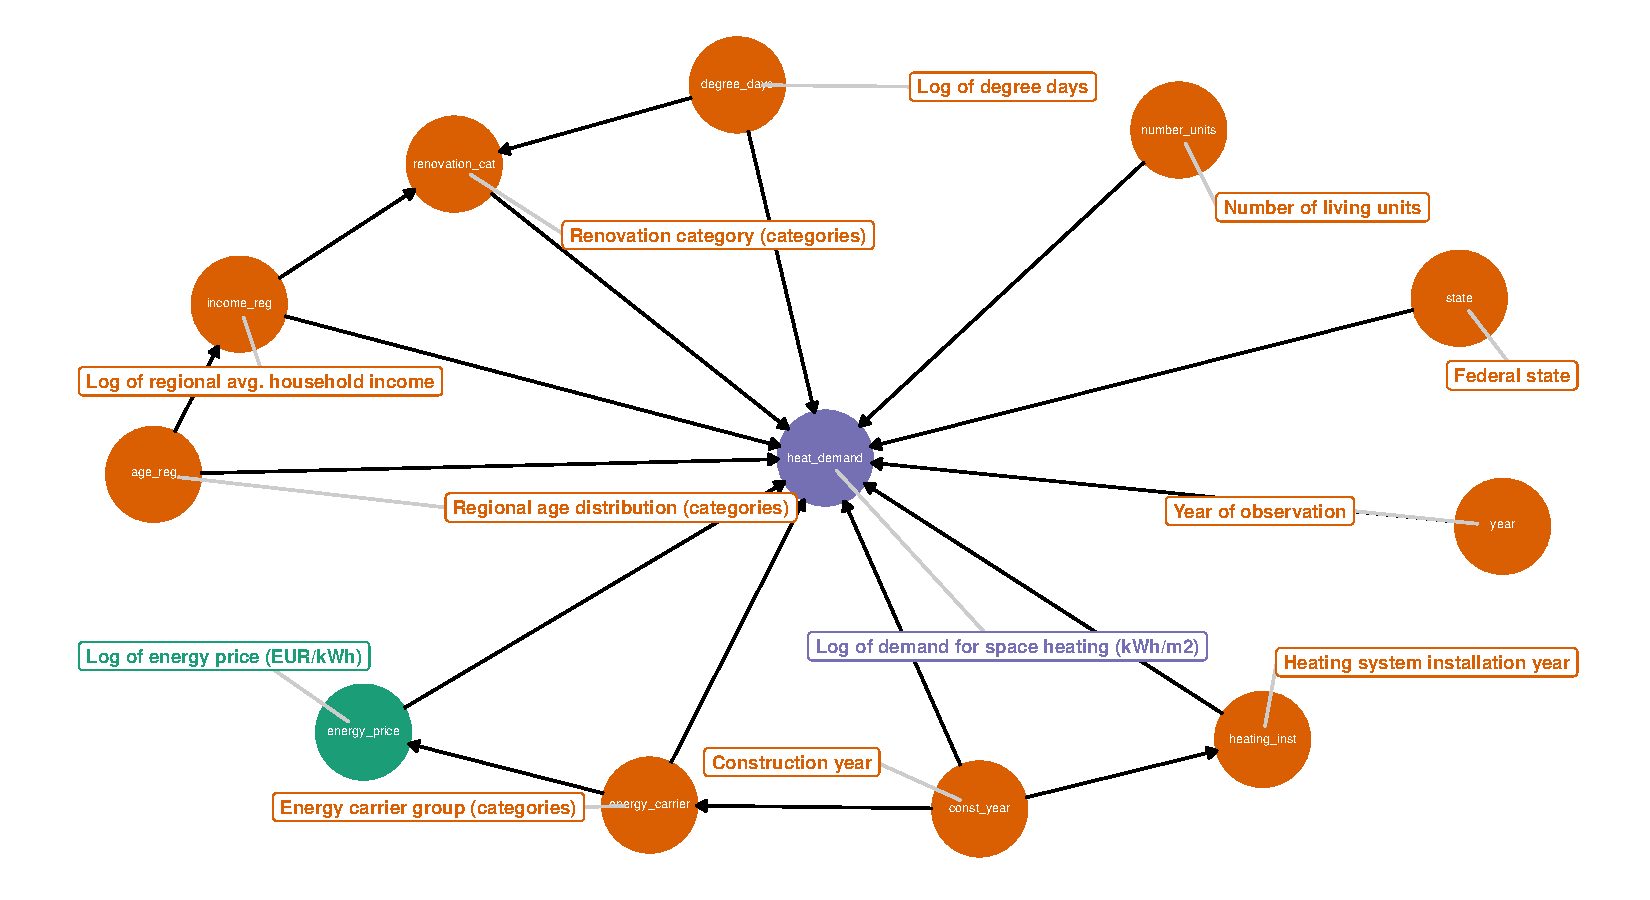
\includegraphics[width=1\linewidth]{figure/conceptual_dag} 

}

\caption{DAG}\label{fig:dag}
\end{figure}
\hypertarget{literature}{%
\chapter{Literature Review}\label{literature}}

The objective of this chapter is to provide an overview of the existing literature on the price elasticity of heating demand. The text is organized as follows. The first part of the chapter focuses on the theoretical interactions between energy prices and energy consumption as well as the resulting effects on greenhouse gas emissions and climate change. The second part of the chapter then summarizes the empirical evidence on price elasticities from the literature.

\hypertarget{literature_intro}{%
\section{Energy prices, energy consumption, and climate change}\label{literature_intro}}

Energy taxation and climate change
- Fuel consumption demand is determined by demand functions that depend primarily on income and prices
- Those who disfavor fuel taxes often claim they are strongly regressive. Earlier studies have shown that this depends on the country studied and on the details of the methods used, for instance if lifetime or temporary income is used, if substitution or other reactions are allowed for in the analysis. There is a tendency to progressivity in low income countries but regressivity in high income countries.
- Indirect channel of long-term price change and anticipation of those changes leading to investments in low-carbon UBA: Remediation measures drawn by lot through the BEHG are partly subsidized through the BEG or the tax incentive and are accounted for there (CO2 price as door opener for subsidy)

Knowing the responsiveness of energy demand to the price allows analysts to predict the effects of price changes or policies that result in price changes---for example, taxes on carbon emissions, or mandates on the share of renewable energy.

The quantity demanded of a good or service depends on multiple factors, such as price, income, and preference. Whenever there is a change in these variables, it causes a change in the quantity demanded of the good or service.

Price elasticity of demand is an economic measure of the sensitivity of demand relative to a change in price. The measure of the change in the quantity demanded due to the change in the price of a good or service is known as price elasticity of demand.

Elasticity estimations:
\begin{itemize}
\tightlist
\item
  Price elasticities for energy is a vast field of literature
\item
  Focus on the behavior of the private households sector and for heating demand as a subset of the larger field of research
\item
  Spatial focuses: many studies on the US and European countries; number of studies especially in China but also in other emerging and less developed countries is rising
\item
  The meta-analysis of Labandeira et al.~(2017) serves as a good starting point for the review of the literature since it compiles the evidence of the past decades on energy price elasticities.
\item
  Previous meta analysis (e.g., xxx) focus solely on gasoline price elasticity studies which is thus unsuitable for the focus of this research.
\item
  At any rate, the large number of surveys on price elasticities of energy demand contrasts with scarce attempts by the literature to summarize these elasticities in a single value through meta-analysis.
\end{itemize}
Short and long run: Economists often distinguish between a short-run response and long-run response when referring to how a household changes its natural gas usage when faced with price and income changes,. The short-run response is defined as a household's natural gas demand response to natural gas price and income changes given their current capital stock of natural gas-using appliances and shell efficiency of the house. The long-run response is defined as a household's response to natural gas prices changes and income changes after the household has had time to change their stock of gas using appliances and house shell efficiency.

Aufhammer results:
We find that the price elasticity of demand for natural gas for households ranges on average from minus 0.23 to minus 0.17. Importantly, we find evidence of heterogeneity in this elasticity along the dimensions of season and income. Both lower-income and higher-income households are essentially inelastic to price in the summer months. In the winter months, however, lower-income households are much more price elastic than higher-income households.

From Csereklyei (2020):

Labandeira et al.~(2017) survey 428 papers published between 1990 and 2016. Most of the surveyed papers use varying econometric techniques, geographic and time scope, resulting in substantial variation in the estimates. Labandeira et al.~(2017) find the average short-run and long-run price elasticities of electricity demand at -0.13 and at -0.37 respectively. Labandeira et al.~(2017) also report that many studies found decreasing elasticities over time. This is similar to the finding of Fouquet (2014), who reports that both the income and price elasticity of energy demand reduced in the UK over the past two hundred years. Several authors, such as Miller and Alberini (2016) Wang and Mogi (2017) and Inglesi-Lotz (2011) report a negative relationship between average prices and the estimated price elasticities in a given year.

Meta-studies are useful in providing us the possible ranges of price and income elasticities, however they might mask large differences arising from the variety of data and methods used. Different levels of aggregation, estimation methods (e.g., panel vs.~cross-sectional, dynamic panel vs.~long-run models), endogeneity and measurement heterogeneity, and price trends all impact on the estimates in the literature (Miller and Alberini, 2016).

\hypertarget{methods}{%
\chapter{Methods}\label{methods}}

Csereklyei (2020):
It is widely anticipated that responses in electricity consumption to changes in prices will be rather slow, as it takes time for energy-using durable stock to change (Miller and Alberini, 2016). Thus, short-run or annual price elasticity estimates are expected to be rather inelastic, while one anticipates significantly larger long-run estimates.

Miller and Alberini (2016) furthermore report that the use of IV estimates can change the reported elasticities by up to 80\%.

All from Labanderira et al.

discrete decision to purchase durable goods that consume energy and the decision to consume energy is rarely considered.
renovations may disturbe the picture the panel data provides

On the other hand, most empirical studies in this area have used single-equation econometric models that require separability re- strictions. This is a severe disadvantage as it is not possible to estimate cross-price effects between different energy products or consider the effects of non-energy products on the price elasticity of energy goods.

Sample period. It is widely accepted that the economic cycle has a strong influence on energy consumption due to income and (indirect cycle-related) price effects. In the case of economic crises, for example, a depression of energy prices may occur; reduced dis- posable income may lead agents to reduce consumption through improvements in energy efficiency, adjustments to other types of consumption or changes towards other more inexpensive energy goods.

From Aufhammer wegen IV approach:
We instrument the utilities' consumer-facing prices with the weekly average spot price of natural gas at a major natural gas distribution hub in Louisiana (the Henry Hub). This instrument is valid, as we know the formula of how utilities pass-through the price (providing a strong first stage), and the price is determined prior to within-bill consumption (strengthening the exclusion restriction).

No change in the energy taxation (Energiesteuergesetz) in the observed period; letzte Neufassung aus 2006 mit Effekten für 2007

\hypertarget{data}{%
\chapter{Data}\label{data}}

Several data sources were used for the analysis presented in this thesis. The section is structured as follows. First, the data sources for the variables used in the analysis are being introduced and shortly described. To structure the description, the variables retrieved from the sources are used. Then, in a second part, the data cleaning process is described and reasoned for where necessary.

\hypertarget{ista_data}{%
\section{Space heat consumption and energy prices}\label{ista_data}}

The data on space heat consumption and energy prices -- which is the backbone of the analysis -- was obtained from a large-scale building-level panel of heating bills made available though the Climate Policy Department at DIW Berlin. The data originates from ista Deutschland GmbH and was provided for scientific use. The sample contains information on an average of 260,000 multi-unit residential buildings in Germany per year and is structured around annual heating bills at the building-level. This means that the smallest buildings observed have two living units; single-family houses with just one unit, on the other hand, are not observed. Spatially, the data have a good coverage spread over all federal states. While the consumption data in the panel already start in 2003, the energy prices are only observable with a more extensive data delivery at the end of 2008. However, since a relevant number of observations billed in 2008 already have the majority of the billing period in 2007, the panel data used ranges from 2007 to 2019.

Consumption data is\ldots{}

Data structure for prices

Additional variables + spatial differenciation

The ista consumption panel serves as a staring point from which the other sources of data are merged to it.

\hypertarget{results}{%
\chapter{Results}\label{results}}

\hypertarget{full_results}{%
\section{Full sample analysis}\label{full_results}}

\hypertarget{full_results_descriptive}{%
\subsection{Descriptive statistics}\label{full_results_descriptive}}

\hypertarget{full_results_regression}{%
\subsection{Regression results}\label{full_results_regression}}

\hypertarget{full_results}{%
\section{Subsample analysis}\label{full_results}}

\hypertarget{full_results_descriptive}{%
\subsection{Descriptive statistics}\label{full_results_descriptive}}

\hypertarget{full_results_regression}{%
\subsection{Regression results}\label{full_results_regression}}

\begingroup\fontsize{10}{12}\selectfont
\begin{longtable}[t]{lr}
\caption{\label{tab:tabletest}Number of flight connections per destination}\\
\toprule
Destination & Number of connections\\
\midrule
\endfirsthead
\caption[]{\label{tab:tabletest}Number of flight connections per destination \textit{(continued)}}\\
\toprule
Destination & Number of connections\\
\midrule
\endhead

\endfoot
\bottomrule
\multicolumn{2}{l}{\rule{0pt}{1em}\textsuperscript{1} This table was created based on the flights dataset.}\\
\multicolumn{2}{l}{\rule{0pt}{1em}\textsuperscript{2} Source: R Packages.}\\
\endlastfoot
Albuquerque International Sunport & 30\\
Bob Hope & 261\\
Boise Air Terminal & 29\\
Charlotte Douglas Intl & 45\\
Chicago Midway Intl & 104\\
\addlinespace
Chicago Ohare Intl & 524\\
Dallas Fort Worth Intl & 441\\
Denver Intl & 905\\
Detroit Metro Wayne Co & 55\\
General Edward Lawrence Logan Intl & 70\\
\addlinespace
George Bush Intercontinental & 228\\
Hartsfield Jackson Atlanta Intl & 410\\
Honolulu Intl & 180\\
John F Kennedy Intl & 137\\
John Wayne Arpt Orange Co & 247\\
\addlinespace
Kahului & 171\\
Kansas City Intl & 89\\
Klamath Falls Airport & 82\\
Kona Intl At Keahole & 90\\
Lihue & 52\\
\addlinespace
Long Beach & 263\\
Los Angeles Intl & 912\\
Mahlon Sweet Fld & 189\\
Mc Carran Intl & 564\\
Metropolitan Oakland Intl & 451\\
\addlinespace
Minneapolis St Paul Intl & 270\\
Newark Liberty Intl & 91\\
Norman Y Mineta San Jose Intl & 574\\
Ontario Intl & 196\\
Palm Springs Intl & 105\\
\addlinespace
Phoenix Sky Harbor Intl & 888\\
Reno Tahoe Intl & 94\\
Roberts Fld & 252\\
Ronald Reagan Washington Natl & 87\\
Sacramento Intl & 404\\
\addlinespace
Salt Lake City Intl & 538\\
San Diego Intl & 265\\
San Francisco Intl & 1265\\
Santa Barbara Muni & 89\\
Seattle Tacoma Intl & 569\\
\addlinespace
Ted Stevens Anchorage Intl & 254\\
Tucson Intl & 90\\
Washington Dulles Intl & 89\\*
\end{longtable}
\endgroup{}

\captionsetup[table]{labelformat=empty,skip=1pt}
\begin{longtable}{lc}
\toprule
\textbf{Variable} & \textbf{N = 2,993,841} \\ 
\midrule
Space heat consumption, eff. [kWh/sqm.] &  \\ 
Mean (SD) & 119 (47) \\ 
Median [Range] & 113 [21, 521] \\ 
Energy price, real [Cents/kWh] &  \\ 
Mean (SD) & 7.01 (2.06) \\ 
Median [Range] & 6.56 [2.00, 99.50] \\ 
Degree days &  \\ 
Mean (SD) & 3,496 (386) \\ 
Median [Range] & 3,445 [2,284, 7,003] \\ 
(Missing) & 3,209 \\ 
Energy carrier category &  \\ 
District heating & 290,010 (9.7\%) \\ 
Gas & 1,806,199 (60\%) \\ 
Oil & 875,945 (29\%) \\ 
Others & 21,687 (0.7\%) \\ 
Building heating surface [sqm.] &  \\ 
Mean (SD) & 694 (1,050) \\ 
Median [Range] & 402 [31, 73,437] \\ 
Building housing units &  \\ 
Mean (SD) & 10 (16) \\ 
Median [Range] & 6 [2, 1,694] \\ 
Regional household income [€] &  \\ 
Mean (SD) & 20,732 (2,925) \\ 
Median [Range] & 20,568 [13,821, 42,555] \\ 
(Missing) & 3,270 \\ 
Regional share retirement [>65 yrs] &  \\ 
Mean (SD) & 0.209 (0.024) \\ 
Median [Range] & 0.207 [0.145, 0.327] \\ 
(Missing) & 6,777 \\ 
 \bottomrule
\end{longtable}
\begin{minipage}{\linewidth}
\emph{This data is simulated}\\ 
\end{minipage}
\hypertarget{discussion}{%
\chapter{Discussion}\label{discussion}}

\hypertarget{conclusion}{%
\chapter{Conclusion}\label{conclusion}}

\appendix

\hypertarget{first-appendix}{%
\chapter{First Appendix}\label{first-appendix}}

\hypertarget{second-appendix}{%
\chapter{Second Appendix}\label{second-appendix}}

(\ldots)

\backmatter

\hypertarget{references}{%
\chapter*{References}\label{references}}
\addcontentsline{toc}{chapter}{References}

\markboth{References}{References}

\noindent

\setlength{\parindent}{-0.20in}

\hypertarget{refs}{}
\begin{CSLReferences}{1}{0}
\leavevmode\vadjust pre{\hypertarget{ref-ageb21}{}}%
AGEB. (2021). \emph{Auswertungstabellen zur Energiebilanz 1990 bis 2020}. Berlin. Retrieved from \url{https://ag-energiebilanzen.de/daten-und-fakten/auswertungstabellen/}

\leavevmode\vadjust pre{\hypertarget{ref-bmwi21}{}}%
BMWi. (2021). \emph{Gesamtausgabe der Energiedaten}. BMWi. Retrieved from \url{https://www.bmwi.de/Redaktion/DE/Binaer/Energiedaten/energiedaten-gesamt-xls.xlsx?__blob=publicationFile\&v=133}

\leavevmode\vadjust pre{\hypertarget{ref-destatis18}{}}%
DESTATIS. (2018). Fernwärmeversorgung 2017: Abgegebene Wärmemenge leicht gesunken. Retrieved January 19, 2022, from \url{https://www.destatis.de/DE/Presse/Pressemitteilungen/2018/11/PD18_434_434.html}

\leavevmode\vadjust pre{\hypertarget{ref-erk20}{}}%
ERK. (2020). \emph{Bericht zur Vorjahresschätzung der deutschen Treibhausgasemissionen für das Jahr 2020}. Retrieved from \url{https://expertenrat-klima.de/content/uploads/2021/04/210415_Bericht_Expertenrat_Klimafragen_2021-2.pdf}

\leavevmode\vadjust pre{\hypertarget{ref-rwi21}{}}%
RWI. (2021). \emph{Anwendungsbilanzen 2020 für den Sektor der privaten Haushalte und den Verkehrssektor in Deutschland}. Retrieved from \url{https://ag-energiebilanzen.de/wp-content/uploads/2020/10/rwi_anwendungsbilanz_2020__priv._hh_und_verkehr__vorl._eb.pdf}

\leavevmode\vadjust pre{\hypertarget{ref-stede_etal20}{}}%
Stede, J., Schütze, F., \& Wietschel, J. (2020). Wärmemonitor 2019: Klimaziele bei Wohngebäuden trotz sinkender CO2-Emissionen derzeit außer Reichweite (Version 2.0). \emph{DIW Wochenbericht}. http://doi.org/\href{https://doi.org/10.18723/DIW_WB:2020-40-1}{10.18723/DIW\_WB:2020-40-1}

\leavevmode\vadjust pre{\hypertarget{ref-techem19}{}}%
Techem. (2019). \emph{Energiekennwerte 2019}. Eschborn: Techem. Retrieved from \url{https://www.techem.com/content/dam/techem/newsroom/studien/Techem-Energiekennwerte-Studie-2019.pdf}

\end{CSLReferences}

% Index?

\end{document}
